\section{Quark-Flavour Physics and CP Violation}
\label{sec:intro_CPV}

%%%%%%%%%%%%%%%%%%%%%%%%%%%%%%%
\subsection{Quark Mixing}
\label{subsec:intro_mixCPV_mix}
%%%%%%%%%%%%%%%%%%%%%%%%%%%%%%%

The Feynman diagrams for the charged weak current that changes the flavour of a quark are shown in Figure~\ref{fig:WCouplings}. The
subscript ``L'' on the quark indicates that only quark states with a left-handed chirality participate in this interaction.
\begin{figure}[hbt]
  {\sffamily %%BoundingBox: -1 -1 61 36 
%%HiResBoundingBox: -1 -1 60.7757 35.86916 

\hspace*{0.03\textwidth}
\begin{fmffile}{graphics/intro/WCouplings/up}
  \fmfframe(8,16)(8,16){
    \begin{fmfgraph*}(60,35)
      \fmfstraight
      \fmftop{id,ou}
      \fmfbottom{iW}
      \fmf{fermion}{id,v,ou}
      \fmf{boson}{iW,v}
      \fmflabel{d$_\text{L}^\prime$}{id}
      \fmflabel{u$_\text{L}^{\phantom{\prime}}$}{ou}
      \fmflabel{W}{iW}
    \end{fmfgraph*}
  }
\end{fmffile}
\hfill
\begin{fmffile}{graphics/intro/WCouplings/charm}
  \fmfframe(8,16)(8,16){
    \begin{fmfgraph*}(60,35)
      \fmfstraight
      \fmftop{id,ou}
      \fmfbottom{iW}
      \fmf{fermion}{id,v,ou}
      \fmf{boson}{iW,v}
      \fmflabel{s$_\text{L}^\prime$}{id}
      \fmflabel{c$_\text{L}^{\phantom{\prime}}$}{ou}
      \fmflabel{W}{iW}
    \end{fmfgraph*}
  }
\end{fmffile}
\hfill
\begin{fmffile}{graphics/intro/WCouplings/top}
  \fmfframe(8,16)(8,16){
    \begin{fmfgraph*}(60,35)
      \fmfstraight
      \fmftop{id,ou}
      \fmfbottom{iW}
      \fmf{fermion}{id,v,ou}
      \fmf{boson}{iW,v}
      \fmflabel{b$_\text{L}^\prime$}{id}
      \fmflabel{t$_\text{L}^{\phantom{\prime}}$}{ou}
      \fmflabel{W}{iW}
    \end{fmfgraph*}
  }
\end{fmffile}
\hspace*{0.03\textwidth}
}
  \caption{Charged-current weak interactions of quarks.}
  \label{fig:WCouplings}
\end{figure}

The primes on the d$_\text{L}^\prime$, s$_\text{L}^\prime$ and b$_\text{L}^\prime$ quarks in the figure indicate that the states that
couple to the W boson are not the quark mass eigenstates. The down-type states in the interaction are given by a rotation of the mass
eigenstates, which is parameterized by the Cabibbo-Kobayashi-Maskawa (CKM) quark-mixing matrix \cite{Kobayashi:1973fv}:
\begin{equation}
  \begin{pmatrix} \text{d}_\text{L}^\prime \\ \text{s}_\text{L}^\prime \\ \text{b}_\text{L}^\prime \end{pmatrix}
    \equiv \VCKM\, \begin{pmatrix} \text{d}_\text{L} \\ \text{s}_\text{L} \\ \text{b}_\text{L} \end{pmatrix}
    \equiv \begin{pmatrix} \Vud & \Vus & \Vub \\ \Vcd & \Vcs & \Vcb \\ \Vtd & \Vts & \Vtb \end{pmatrix}
           \begin{pmatrix} \text{d}_\text{L} \\ \text{s}_\text{L} \\ \text{b}_\text{L} \end{pmatrix}
    \ .
\end{equation}
Diagrams with W-boson vertices in which one of the three mass eigenstates is selected are proportional to the appropriate matrix element
$V_{ij}$. A similar mechanism applies for mixing of leptons \cite{Pontecorvo:1957cp,*Pontecorvo:1957qd,*Maki:1962mu,*Pontecorvo:1967fh}.

The CKM matrix is a unitary complex matrix. The number of independent parameters in the matrix is limited by the constraint of unitarity
and by the fact that part of the complex phases of the matrix elements can be absorbed in the arbitrary phases of the quark fields.
Representation of the CKM matrix in terms of the four remaining parameters is convention dependent. A commonly used choice is the
\emph{Wolfenstein parameterization} with real-valued $\Vud$, $\Vus$, $\Vcb$, and $\Vtb$ and a single complex phase entering in the other
elements \cite{Wolfenstein:1983yz,*Chau:1984fp,*Buras:1994ec}. Four real parameters, $\lam$, $A$, $\rho$, and $\eta$, are then
defined by
\begin{equation}
  \begin{gathered}
    \lam \equiv \frac{|\Vus|}{\sqrt{|\Vud|^2 + |\Vus|^2}}
      \quad
      A\lam^2 \equiv \frac{|\Vcb|}{\sqrt{|\Vud|^2 + |\Vus|^2}}
      \quad
      A\lam^3(\rho+i\eta) \equiv \Vub[*]
      \ \ .
  \end{gathered}
\end{equation}

The Wolfenstein parameterization of the CKM matrix is motivated by the orders of magnitude of matrix elements. The magnitudes of the
diagonal elements $\Vud$, $\Vcs$ and $\Vtb$, which describe the coupling between up-type and down-type quarks of the same generation, are
approximately equal to one. Magnitudes of the couplings between the first and second generation are between a factor four and five smaller:
$|\Vus|\approx|\Vcd|\approx\lam\approx0.23$ \cite{Charles:2004jd,Bona:2005vz}.

Couplings between the second and third and between the first and third generation are suppressed by factors $\lam^2$ and $\lam^3$,
respectively: $|\Vcb|\approx|\Vts|\approx A\lam^2\approx0.04$, $|\Vub|=A\lam^3|\rho+i\eta|\approx0.004$, and $|\Vtd|\approx
A\lam^3|1-\rho-i\eta|\approx0.009$. In this form of the Wolfenstein parameterization the complex phase is introduced with the parameters
$\rho\approx0.13$ and $\eta\approx0.36$, where $\arg(\Vub[*])=\arg(\rho+i\eta)\approx70^\circ$.

%Expanding the CKM matrix in terms of the small parameter $\lam$ within the Wolfenstein parameterization yields
%\begin{equation}
%  \begin{split}
%    \VCKM =& \begin{pmatrix}
%               1 - \tfrac{1}{2}\lam^2 - \tfrac{1}{8}\lam^4  &  0  &  0 \\
%               0  &  1 - \tfrac{1}{2}\lam^2 - \tfrac{1}{8}\lam^4 (1+4A^2) & 0 \\
%               0  &  0  &  1 - \tfrac{1}{2}A^2\lam^4
%             \end{pmatrix} \\
%          &+ \phantom{A}\lam\phantom{^2}
%            \begin{pmatrix}
%               \phantom{-}0                                   &  1            &  0     \\
%               -\left[1 - \tfrac{1}{2}A^2\lam^4(1-2r)\right]  &  \quad0\quad  &  \ 0\  \\
%               \phantom{-}0                                   &  0            &  0
%            \end{pmatrix} \\
%          &+ A\lam^2
%            \begin{pmatrix}
%               0     &  0                                             &  0    \\
%               0     &  0                                             &  1    \\
%               \ 0\  &  -\left[ 1 - \tfrac{1}{2}\lam^2(1-2r) \right]  &  \ 0\
%            \end{pmatrix} \\
%          &+ A\lam^3
%            \begin{pmatrix}
%               0                                &  \quad0\quad  &  r^*\  \\
%               0                                &  0            &  0     \\
%               1 - (1 - \tfrac{1}{2}\lam^2)\,r  &  0            &  0
%            \end{pmatrix}
%           + \mathcal{O}(\lam^6)
%    \ .
%  \end{split}
%\end{equation}

The CKM matrix can be expanded in terms of the small parameter $\lam$. Neglecting terms of order $\lam^4$ and higher relative to the
leading term for each element, it is approximated by \cite{Charles:2004jd}
\begin{equation}
  \label{eq:CKMApprox}
  \VCKM \approx
    \begin{pmatrix}
      c                  &  \lam                           &  \!\! A\lam^3\,r^* \\
      -\lam              &  c                              &  A\lam^2           \\
      A\lam^3(1 - c\,r)  &  \!\! -A\lam^2 (c + \lam^2\,r)  &  1
    \end{pmatrix}
    \ ,
\end{equation}
where $c\equiv1 - \tfrac{1}{2}\lam^2$ and $r\equiv\rho+i\eta$.

Notice that only the elements $\Vub$, $\Vtd$ and $\Vts$ have non-vanishing imaginary parts in this approximation. In $\Vts$ the parameter $r$ is suppressed by a
factor $\lam^2$, which makes the imaginary part of this element much smaller than the real part. For $\Vcd$ and $\Vcs$ the suppression
factors are $\lam^4$ and $\lam^6$, respectively, which results in vanishing imaginary parts.


%%%%%%%%%%%%%%%%%%%%%%%%%%%%%%%
\subsection{CP Violation}
\label{subsec:intro_mixCPV_CPV}
%%%%%%%%%%%%%%%%%%%%%%%%%%%%%%%

The Standard Model mixing formalism was introduced for quarks, but it also applies to antiquarks. A CP operation on the states in
Figure~\ref{fig:WCouplings} results in the interactions of right-handed antiquark states with the W boson.

In the transformation from quarks to antiquarks the CKM-matrix elements in the weak interaction states are replaced with their complex
conjugates. If there were no complex phase in the CKM matrix, its elements would be real and the weak interactions of quarks would be
invariant under the CP transformation. Introducing a complex phase breaks this invariance and gives rise to CP violation. The CKM matrix is
the only source of CP violation in the Standard Model with massless leptons.

Although the complex phase in the CKM matrix formally breaks CP invariance, CP-violating phenomena cannot be observed directly in processes
that are described by a single diagram with W-boson interactions. The magnitude of a diagram is squared to obtain the corresponding
observable probability, which makes its phase unobservable.

CP violation can only be observed in processes where two or more amplitudes with different CKM elements interfere. The CKM elements then
introduce a different \emph{weak phase} for each contribution, which changes sign between CP-conjugate processes. Differences between the
weak phases do affect the observable magnitude of the total amplitude if the contributing amplitudes also have different \emph{strong
phases}, which do not change sign under a CP transformation.

This can be illustrated by considering two interfering amplitudes $A_1$ and $A_2$ with CKM factors $F_1$ and $F_2$. The asymmetry between
the squared magnitudes for CP-conjugate processes is then given by
\begin{equation}
  \label{eq:interference}
  \begin{split}
    A_\text{CP} &\equiv \frac{|\Af[]|^2 - |\Abarf[]|^2}{|\Af[]|^2 + |\Abarf[]|^2}
                 = \frac{|F_1\,A_1 + F_2\,A_2|^2 - |F_1^*\,A_1 + F_2^*\,A_2|^2}{|F_1\,A_1 + F_2\,A_2|^2 + |F_1^*\,A_1 + F_2^*\,A_2|^2} \\
                &= \frac{-2 R\, \sin(\Delta\delta)\, \sin(\Delta\phi)}{1 + R^2 + 2 R\, \cos(\Delta\delta)\, \cos(\Delta\phi)}
                   \ ,
  \end{split}
\end{equation}
where $R\equiv\frac{|F_2|\,|A_2|}{|F_1|\,|A_1|}$, $\Delta\delta\equiv\arg(A_2)-\arg(A_1)$ and $\Delta\phi\equiv\arg(F_2)-\arg(F_1)$. Notice
that the CP asymmetry vanishes if there is no weak phase difference $\Delta\phi$, but also if there is no strong phase difference
$\Delta\delta$. The size of the asymmetry also depends on the relative magnitudes of the amplitudes and CKM factors. The asymmetry vanishes
in case the $|F_2|\,|A_2|$ is much smaller than $|F_1|\,|A_1|$.

To construct convention-independent measures of CP violation in quark interactions, the CKM-matrix unitarity constraints are used. The
unitarity relation $\VCKM[\dagger]\VCKM = \VCKM\VCKM[\dagger] = \mathbb{1}$ gives nine constraints. Six of these are orthogonality
relations, two of which are given by
\begin{subequations}
  \label{eq:unitConstraints}
  \begin{align}
    \text{``d--b'':} & \quad \Vud\Vub[*] + \Vcd\Vcb[*] + \Vtd\Vtb[*] = 0 \nonumber \\
    \label{eq:unitConstraints_d}
    &\qquad\qquad\qquad \implies\ 1 + \frac{\Vud\Vub[*]}{\Vcd\Vcb[*]} + \frac{\Vtd\Vtb[*]}{\Vcd\Vcb[*]} = 0 \\
    \text{``s--b'':} & \quad \Vus\Vub[*] + \Vcs\Vcb[*] + \Vts\Vtb[*] = 0 \nonumber \\
    \label{eq:unitConstraints_s}
    &\qquad\qquad\qquad \implies\ 1 + \frac{\Vus\Vub[*]}{\Vcs\Vcb[*]} + \frac{\Vts\Vtb[*]}{\Vcs\Vcb[*]} = 0 \ .
  \end{align}
\end{subequations}

Notice that the phases of the combinations of four CKM elements that appear in Equation~\ref{eq:unitConstraints} are of the form $\arg(
V^{\phantom{*}}_{ij} V^{\phantom{*}}_{kl} V^{*}_{il} V^{*}_{kj} )$. Each of the quark indices in this expression appears twice; once for a
matrix element and once for the complex conjugate of a matrix element. Absorbing CKM phases in the quark fields gives opposite phase shifts
for the two corresponding elements, which makes the phase of the four-element combination invariant and convention independent.

\begin{figure}[tb]
  \centering
  \begin{subfigure}{0.475\textwidth}
    \raggedright
    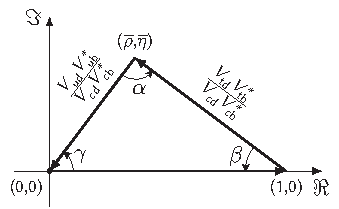
\includegraphics{graphics/intro/tikz/b-d-triangle}
    \caption{}
    \label{fig:unitTriangles_bd}
  \end{subfigure}%
  \begin{subfigure}{0.525\textwidth}
    \raggedleft
    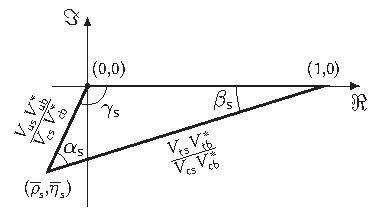
\includegraphics{graphics/intro/tikz/b-s-triangle}
    \caption{}
    \label{fig:unitTriangles_bs}
  \end{subfigure}
  \caption{CKM-unitarity triangles. (a) d--b triangle, corresponding to Equation~\ref{eq:unitConstraints_d}. (b) s--b triangle,
           corresponding to Equation~\ref{eq:unitConstraints_s}.}
  \label{fig:unitTriangles}
\end{figure}

The three terms in each of the orthogonality relations can be used to construct a triangle in the complex plane. The resulting
\emph{unitarity triangles} are schematically shown in Figure~\ref{fig:unitTriangles}. Figure~\ref{fig:unitTriangles_bd} shows the
\emph{d--b triangle}, which corresponds to Equation~\ref{eq:unitConstraints_d}. Its sides are defined by the CKM elements for the couplings
of the up-type quarks and the down/beauty quarks. The angles $\alpha$, $\beta$ and $\gamma$ are defined by
\begin{equation}
  \label{eq:bdAnglesDef}
  \alpha \equiv \arg\left( -\frac{\Vtd\Vtb[*]}{\Vud\Vub[*]} \right)
  \quad
  \beta  \equiv \arg\left( -\frac{\Vcd\Vcb[*]}{\Vtd\Vtb[*]} \right)
  \quad
  \gamma \equiv \arg\left( -\frac{\Vud\Vub[*]}{\Vcd\Vcb[*]} \right)
  \ .
\end{equation}
The coordinates of the triangle apex are defined as $(\rhobar, \etabar)$.

Equation~\ref{eq:unitConstraints_s} gives the \emph{s--b triangle} in Figure~\ref{fig:unitTriangles_bs}. It is defined in a
similar way as the d--b triangle, but its apex has negative real and imaginary coordinates $(\rhosbar, \etasbar)$. The angles $\as$, $\bs$
and $\gs$ are given by
\begin{equation}
  \label{eq:bsAnglesDef}
  \as \equiv \arg\left( -\frac{\Vus\Vub[*]}{\Vts\Vtb[*]} \right)
  \quad
  \bs \equiv \arg\left( -\frac{\Vts\Vtb[*]}{\Vcs\Vcb[*]} \right)
  \quad
  \gs \equiv \arg\left( -\frac{\Vcs\Vcb[*]}{\Vus\Vub[*]} \right)
  \ .
\end{equation}

In Figure~\ref{fig:unitTriangles} the sides of the s--b and d--b triangles were scaled with factors $\Vcd\Vcb[*]$ and $\Vcs\Vcb[*]$,
respectively, to make the first side lie between 0 and 1. Without this scaling, the surface areas of the six possible unitarity triangles
are equal and provide a convention-independent measure of the CP violation that is introduced by the CKM matrix. The areas are given by
half of the \emph{Jarlskog invariant} ($J$) \cite{Jarlskog:1985ht}, which is defined by
\begin{equation}
  \Im( V^{\phantom{*}}_{ij} V^{\phantom{*}}_{kl} V^{*}_{il} V^{*}_{kj} ) \equiv J\; \sum_{m,n} \epsilon_{ikm}\,\epsilon_{jln}
  \ ,
\end{equation}
where $\epsilon$ is the Levi-Civita symbol.

Using the Wolfenstein parameterization and neglecting terms of relative order $\lam^4$ and higher (Equation~\ref{eq:CKMApprox}), the
Jarlskog invariant can be expressed as
\begin{equation}
  J \approx A^2\, \lam^6\, (1-\tfrac{1}{2}\lam^2)\, \eta
  \ .
\end{equation}
Its experimental value is approximately 3\tenpowmult{--5}~\cite{Charles:2004jd,Bona:2005vz}. This value is four orders of magnitude smaller
than the theoretical maximum of $\frac{\text{1}}{\text{6}\sqrt{\text{3}}}$\textapprox0.1 given by unitarity.

In the same relative $\lam^3$ approximation, the only CKM-matrix elements with imaginary parts are $\Vub$, $\Vtd$ and $\Vts$. Using the
approximations of the matrix elements from Equation~\ref{eq:CKMApprox} and the angle definitions from Equations~\ref{eq:bdAnglesDef} and
\ref{eq:bsAnglesDef}, the angles $\gamma$, $\beta$, and $\bs$ are approximated by
\begin{subequations}
  \label{eq:CKMAnglesApprox}
  \begin{alignat}{2}
    \label{eq:CKMGammaApprox}
    \gamma \approx \pi - \gs &\approx \phantom{-}\arg(\Vub[*])
      &&\approx \arctan\left( \frac{\eta}{\rho} \right) \\
    \label{eq:CKMBetaApprox}
    \beta                    &\approx           -\arg(\Vtd)
      &&\approx \arctan\left( \frac{(1-\tfrac{1}{2}\lam^2)\,\eta}{1 - (1-\tfrac{1}{2}\lam^2)\,\rho} \right) \\
    \label{eq:CKMBetasApprox}
    \bs                      &\approx \phantom{-}\arg(-\Vts)
      &&\approx \arctan\left( \frac{\lam^2\,\eta}{1 - \tfrac{1}{2}\lam^2 + \lam^2\rho} \right)
    \ .
  \end{alignat}
\end{subequations}
Expanding the expressions for the angles $\alpha$ and $\alpha_{\text{s}}$ in the same way gives the expected relations between the three
angles in a triangle:
\begin{subequations}
  \begin{alignat}{2}
    \alpha &\approx\, \pi + \arg(\Vtd)  - \arg(\Vub[*]) \,&&\approx\, \pi - \beta - \gamma \\
    \as    &\approx\, \arg(\Vub[*]) - \arg(-\Vts)       \,&&\approx\, \pi - \bs   - \gs
    \ .
  \end{alignat}
\end{subequations}

The experimental values of the CKM angles can be determined by a global fit of the Standard Model to all relevant experimental data. There
are two groups doing such a fit, using different statistical methods and slightly different sets of input data. With the experimental data
that were available in the spring of 2013, the CKMfitter Group finds~\cite{Charles:2004jd}
\begin{equation}
  \label{eq:CKMAnglesCKMf}
  \gamma = (69.7^{+1.3}_{-2.8})^\circ \qquad \beta = (21.8^{+0.8}_{-0.7})^\circ \qquad \bs = (1.05\pm0.04)^\circ
  \ .
\end{equation}

Figures~\ref{fig:unitTriangleMeas_db} and \ref{fig:unitTriangleMeas_sb} show the resulting CKMfitter unitarity triangles, together with the
constrains on the coordinates of the triangle apices. At lowest order in $\lambda$ the apices of the d--b and s--b triangles are given by
$(\rhobar, \etabar)$\textapprox$(\rho, \eta)$ and $(\rhosbar, \etasbar)$\textapprox$(-\lam^2\,\rho,\ -\lam^2\,\eta)$, respectively.
Constraints from the fit are given by
\begin{equation}
  \label{eq:CKMApicesCKMf}
  \begin{aligned}
    (\rhobar, \etabar)   &= (+0.129^{+0.018}_{-0.009},\ +0.348^{+0.012}_{-0.012}) \\[0.3em]
    (\rhosbar, \etasbar) &= (-0.0068^{+0.0005}_{-0.0010},\ -0.0185^{+0.0006}_{-0.0007})
  \end{aligned}
\end{equation}

\begin{figure}[htbp]
  \centering
  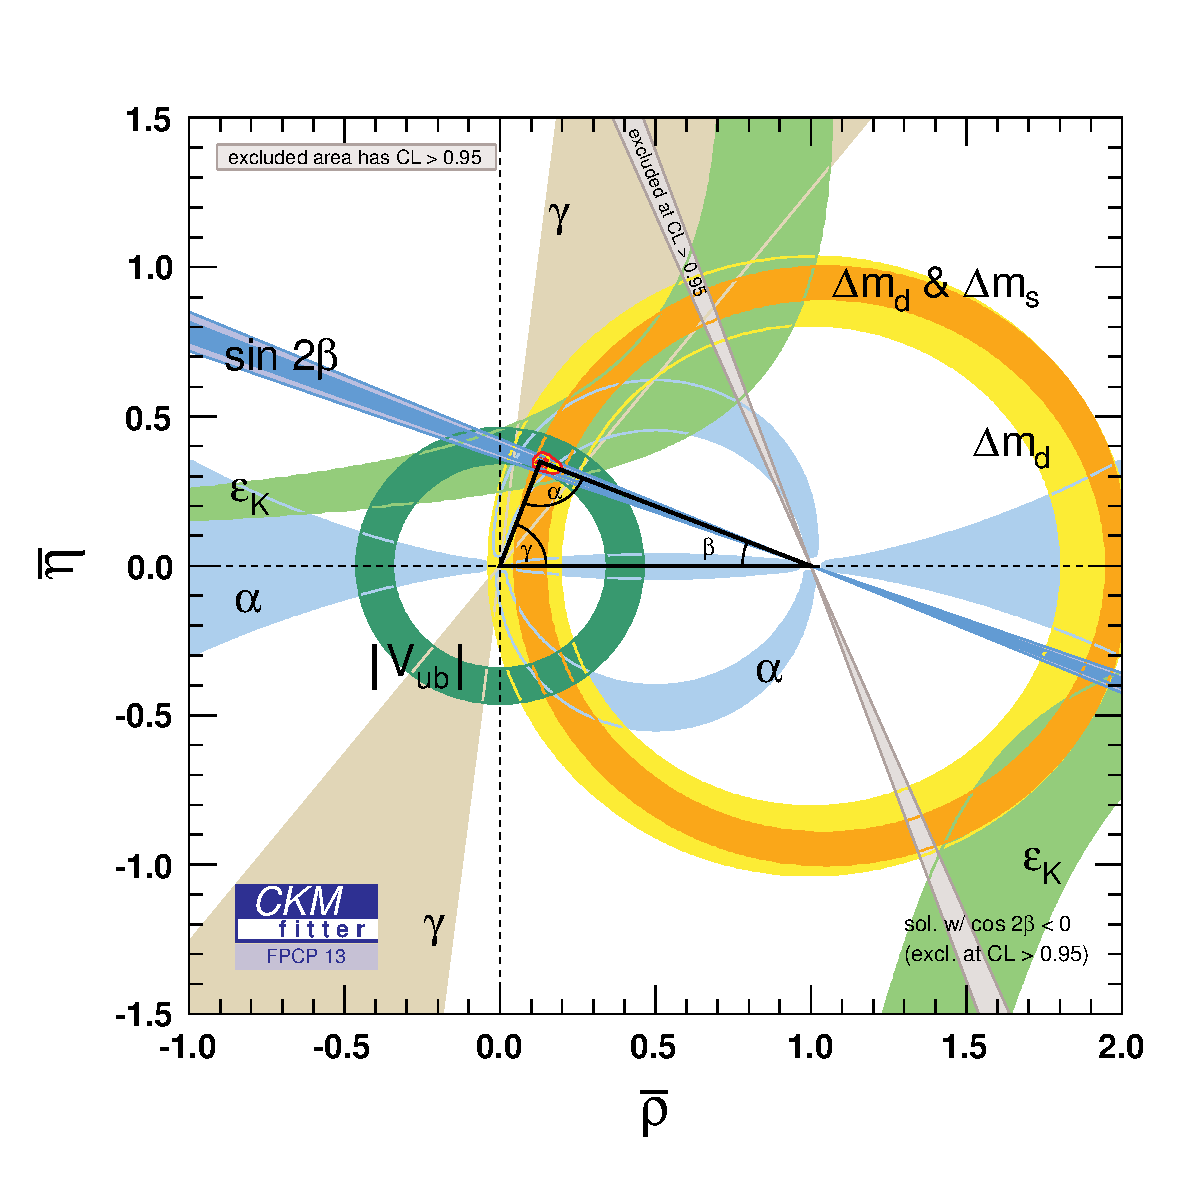
\includegraphics[trim=5mm 2mm 3mm 15mm, clip=true, width=0.8\textwidth]{graphics/intro/rhoeta_large_CMYK}
  \caption{Constraints on the d--b unitarity triangle resulting from the global Standard-Model fit by the CKMfitter Group
           \cite{Charles:2004jd}. The fit estimates the coordinates of the triangle apex in the complex plane, which is given by the
	   parameters $\rhobar\approx\rho$ and $\etabar\approx\eta$.
           Constraints on these parameters from the measurements that are input to the fit are shown as the coloured bands.}
  \label{fig:unitTriangleMeas_db}
\end{figure}

\begin{figure}[htbp]
  \centering
  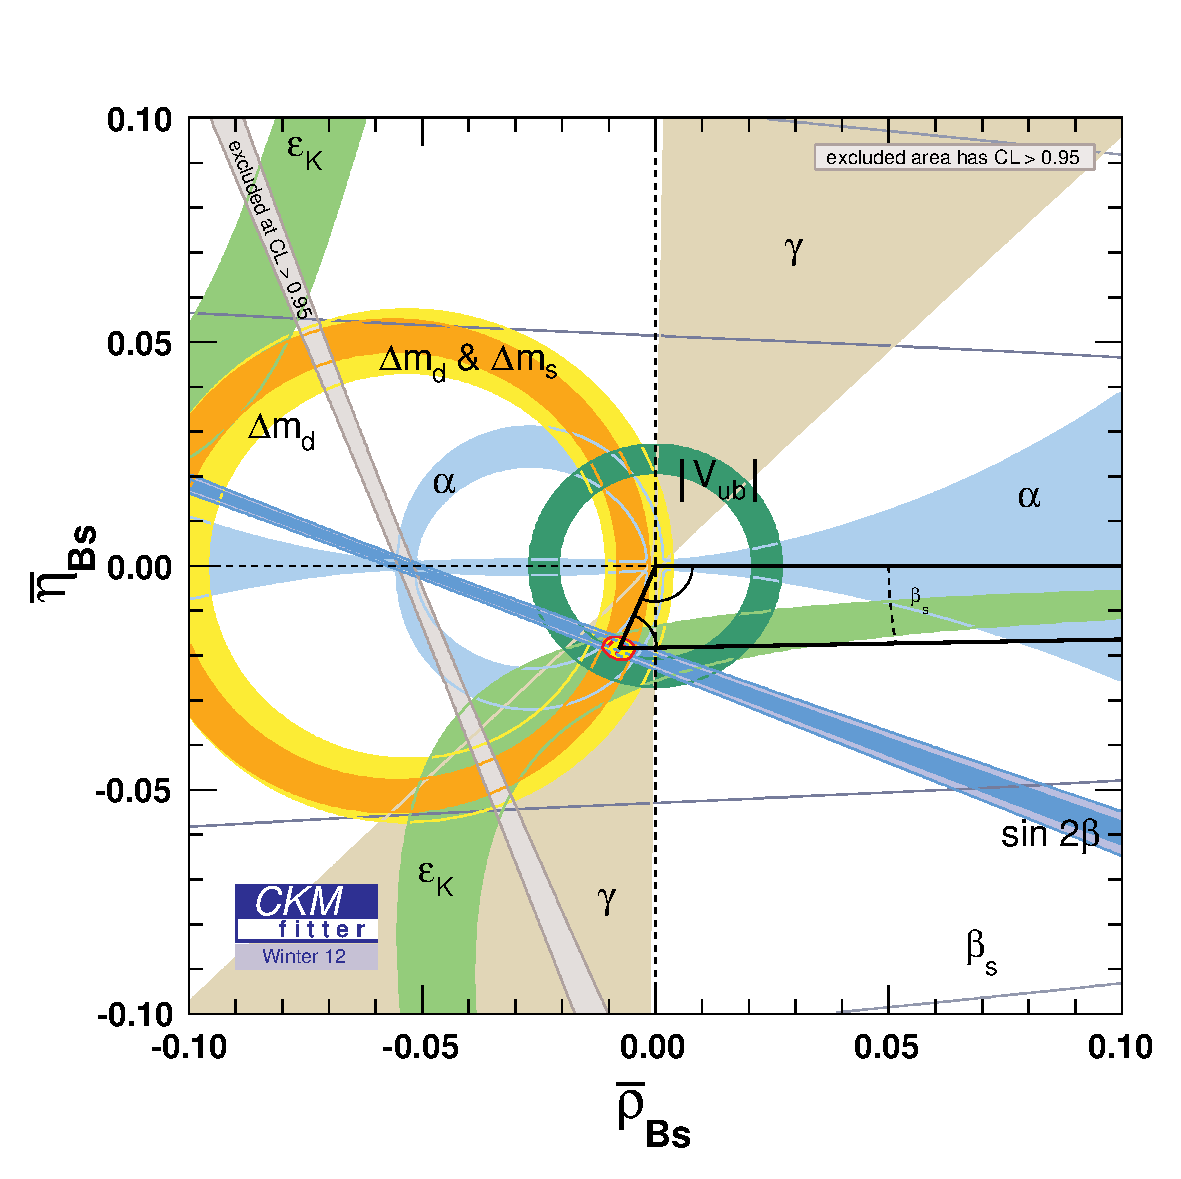
\includegraphics[trim=6mm 2mm 2mm 15mm, clip=true, width=0.8\textwidth]{graphics/intro/rhoBsetaBs_large_global_CMYK}
  \caption{Constraints on the s--b unitarity triangle resulting from the global Standard-Model fit by the CKMfitter Group
           \cite{Charles:2004jd}. The fit estimates the coordinates of the triangle apex in the complex plane, which is given by the
	   parameters $\rhosbar\approx-\lam^2\,\rho$ and $\etasbar\approx-\lam^2\,\eta$.
           Constraints on these parameters from the measurements that are input to the fit are shown as the coloured bands.}
  \label{fig:unitTriangleMeas_sb}
\end{figure}

The UTfit Collaboration finds slightly different values for the angles with the data available by summer 2013~\cite{Bona:2005vz}:
\begin{equation}
  \label{eq:CKMAnglesUTf}
  \gamma = (70.3\pm3.5)^\circ \qquad \beta = (22.0\pm0.9)^\circ \qquad \bs = (1.07\pm0.04)^\circ
  \ .
\end{equation}

Quark-flavour changing interactions and the CKM picture of CP violation provide excellent probes for testing the Standard Model. There are,
for example, measurements that yield one of the CKM angles if only Standard Model processes are considered. If such a measurement gives a
deviation from the value predicted by a global fit or from the value from another measurement, this would be clear evidence for physics
beyond the Standard Model.

As will be discussed in the next section, the CP-violation measurement in the \BstoJpsiphi{} decay yields the phase $\phis$. This phase is
approximately equal to --2$\bs$ in the Standard Model. The value of the angle $\bs$ is very small, since the imaginary part of $\Vts$ is
proportional to a factor $\lam^2$ (see Equations~\ref{eq:CKMApprox} and \ref{eq:CKMBetasApprox}). Even if contributions of unknown new
physics to $\phis$ are small, they could still significantly add to the suppressed Standard Model contribution.
